% 第15章第5节：正交约束下的矩阵逼近（正交逼近的最优解、旋转约束下的逼近）。

\section{正交约束下的矩阵逼近}
\label{sec:matrix-approximation-orthogonal}

前面的约束是秩预算，本节把约束换成正交性。给定方阵$\bm A\in\mathbb R^{d\times d}$，在全部正交矩阵$\bm R$（$\bm R^\top\bm R=\bm I$）中寻找离$\bm A$最近的一个，误差仍用Frobenius范数。正交矩阵保持长度，所以问题是：哪一个保长作用最接近给定的线性作用？例如测得的旋转因噪声不再正交时，就要把它修正为最近的正交矩阵。

正交矩阵组成的集合不是线性子空间，也不由秩描述，前两节的投影化归不能沿用。第~\ref{chap:polar-decomposition}章已经构造了极分解$\bm A=\bm W\bm H$的正交因子$\bm W$；本节证明它正是所求的最近正交矩阵，再讨论要求$\det\bm R=1$时答案怎样改变。

\subsection{正交逼近的最优解}
\label{sec:matrix-approximation-orthogonal-optimum}

\subsubsection{主要思想}

\paragraph{化为迹最大}
要解的问题是
\begin{equation}
 \min_{\bm R^\top\bm R=\bm I}\lVert\bm A-\bm R\rVert_{\mathrm F}^2 .
 \label{eq:matrix-approximation-orthogonal-problem}
\end{equation}
先把目标展开。Frobenius范数的平方是矩阵与自身的迹内积，
\[
 \begin{aligned}
 \lVert\bm A-\bm R\rVert_{\mathrm F}^2
 &=\operatorname{tr}\bigl((\bm A-\bm R)^\top(\bm A-\bm R)\bigr)\\
 &=\lVert\bm A\rVert_{\mathrm F}^2-2\operatorname{tr}(\bm R^\top\bm A)+\lVert\bm R\rVert_{\mathrm F}^2 ,
 \end{aligned}
\]
这里用了$\operatorname{tr}(\bm A^\top\bm R)=\operatorname{tr}(\bm R^\top\bm A)$。

约束使最后一项成为常数：对任意正交矩阵$\bm R$，
\[
 \lVert\bm R\rVert_{\mathrm F}^2=\operatorname{tr}(\bm R^\top\bm R)=\operatorname{tr}\bm I=d .
\]
于是
\begin{equation}
 \lVert\bm A-\bm R\rVert_{\mathrm F}^2
 =\lVert\bm A\rVert_{\mathrm F}^2+d-2\operatorname{tr}(\bm R^\top\bm A),
 \label{eq:matrix-approximation-orthogonal-expansion}
\end{equation}
前两项与$\bm R$无关，距离最小等价于在正交矩阵中最大化$\operatorname{tr}(\bm R^\top\bm A)$。

以$d=2$为例按元素写出这个目标：
\[
 \operatorname{tr}(\bm R^\top\bm A)
 =r_{1,1}a_{1,1}+r_{2,1}a_{2,1}+r_{1,2}a_{1,2}+r_{2,2}a_{2,2}.
\]
它是$\bm R$与$\bm A$对应元素乘积之和，关于$\bm R$是线性的。第~\ref{sec:ls-rank-k-trace}节选择子空间时的目标$\operatorname{tr}(\bm Y^\top\bm G\bm Y)$关于$\bm Y$是二次的，那里的迹极值界不能直接搬用，需要重新给出上界。

\paragraph{换到奇异向量坐标}
线性目标的上界来自SVD。代入$\bm A=\bm U\bm\Sigma\bm V^\top$，并令
\[
 \bm Z=\bm U^\top\bm R\bm V .
\]
$\bm Z$是正交矩阵的乘积，仍然正交，且$\bm R=\bm U\bm Z\bm V^\top$；$\bm R$取遍全部正交矩阵时，$\bm Z$也取遍全部正交矩阵。由迹的循环性，
\[
 \operatorname{tr}(\bm R^\top\bm A)
 =\operatorname{tr}(\bm V\bm Z^\top\bm U^\top\bm U\bm\Sigma\bm V^\top)
 =\operatorname{tr}(\bm Z^\top\bm\Sigma),
\]
问题变成在正交矩阵$\bm Z$中最大化$\operatorname{tr}(\bm Z^\top\bm\Sigma)$。

仍以$d=2$为例。$\bm\Sigma=\operatorname{diag}(\sigma_1,\sigma_2)$右乘到$\bm Z^\top$上，只把第$i$列乘以$\sigma_i$：
\[
 \bm Z^\top\bm\Sigma
 =\begin{bmatrix}z_{1,1}\sigma_1&z_{2,1}\sigma_2\\z_{1,2}\sigma_1&z_{2,2}\sigma_2\end{bmatrix}.
\]
取对角元求和，得
\[
 \operatorname{tr}(\bm Z^\top\bm\Sigma)=\sigma_1z_{1,1}+\sigma_2z_{2,2}.
\]
一般地，
\[
 \operatorname{tr}(\bm Z^\top\bm\Sigma)=\sum_{i=1}^d\sigma_iz_{i,i},
\]
目标只用到$\bm Z$的对角元，每个对角元以对应的奇异值为权重。

\paragraph{由SVD读出最优正交矩阵}
$\bm Z$的每一列都是单位向量，所以每个分量的绝对值不超过$1$，特别地$z_{i,i}\leq1$。奇异值非负，于是逐项有$\sigma_iz_{i,i}\leq\sigma_i$，求和得
\[
 \operatorname{tr}(\bm R^\top\bm A)\leq\sum_{i=1}^d\sigma_i .
\]
$\bm Z=\bm I$时每个对角元都等于$1$，上界取到；换回原来的变量，就是
\begin{equation}
 \bm R_\star=\bm U\bm V^\top .
 \label{eq:matrix-approximation-orthogonal-optimum}
\end{equation}
最优正交矩阵直接由SVD的两个正交因子相乘读出，奇异值只决定误差的大小。下面的定理给出完整的结论，并把它与极分解联系起来。

\begin{theorem}[最佳正交逼近]
\label{thm:ls-best-orthogonal-approximation}
设$\bm A\in\mathbb R^{d\times d}$有SVD$\bm A=\bm U\bm\Sigma\bm V^\top$。对任意正交矩阵$\bm R$，
\begin{equation}
 \operatorname{tr}(\bm R^\top\bm A)\leq\sum_{i=1}^d\sigma_i ,
 \label{eq:matrix-approximation-orthogonal-trace-bound}
\end{equation}
取$\bm R=\bm U\bm V^\top$时等号成立。因此
\begin{equation}
 \min_{\bm R^\top\bm R=\bm I}\lVert\bm A-\bm R\rVert_{\mathrm F}^2
 =\sum_{i=1}^d(\sigma_i-1)^2 ,
 \label{eq:matrix-approximation-orthogonal-min-error}
\end{equation}
最小值由极分解的正交因子达到。$\bm A$可逆时最优解唯一，就是$\bm W=\bm A(\bm A^\top\bm A)^{-1/2}$。
\end{theorem}
\begin{proof}
令$\bm Z=\bm U^\top\bm R\bm V$。由迹的循环性，
\[
 \operatorname{tr}(\bm R^\top\bm A)
 =\operatorname{tr}(\bm V\bm Z^\top\bm U^\top\bm U\bm\Sigma\bm V^\top)
 =\operatorname{tr}(\bm Z^\top\bm\Sigma)
 =\sum_{i=1}^d\sigma_iz_{i,i}.
\]
$\bm Z$的每一列都是单位向量，所以$|z_{i,i}|\leq1$；又$\sigma_i\geq0$，故$\sigma_iz_{i,i}\leq\sigma_i$，求和即得上界。$\bm R=\bm U\bm V^\top$时$\bm Z=\bm I$，等号成立。

由式~\eqref{eq:matrix-analysis-frobenius-norm}，$\lVert\bm A\rVert_{\mathrm F}^2=\sum_i\sigma_i^2$，代入展开式得最小值
\[
 \sum_{i=1}^d\sigma_i^2+d-2\sum_{i=1}^d\sigma_i
 =\sum_{i=1}^d(\sigma_i-1)^2 .
\]
由定理~\ref{thm:ls-polar-general}，$\bm U\bm V^\top$是极分解的正交因子。

设$\bm A$可逆，则全部$\sigma_i>0$。等号要求每一项$\sigma_iz_{i,i}=\sigma_i$，即$z_{i,i}=1$；单位列向量$\bm Z_{:,i}$的第$i$个分量为$1$，其余分量只能为零，于是$\bm Z_{:,i}=\bm e_i$，$\bm Z=\bm I$，$\bm R=\bm U\bm V^\top$。由定理~\ref{thm:ls-polar-invertible}，它就是$\bm W$。
\end{proof}

\paragraph{误差的含义}
去掉伸缩得到的正交因子，同时解决了“离$\bm A$最近的正交矩阵”这个问题；这一结论称为\term{最佳正交逼近}（best orthogonal approximation）。

误差$\sum_i(\sigma_i-1)^2$逐个比较奇异值与$1$。正交矩阵的奇异值全为$1$，最佳正交逼近保留$\bm A$的两组奇异方向，只把$\bm\Sigma$换成$\bm I$：
\[
 \bm A=\bm U\bm\Sigma\bm V^\top\ \longrightarrow\ \bm R_\star=\bm U\bm I\bm V^\top .
\]

\paragraph{奇异情形}
$\bm A$奇异时，最优解一般不唯一，而且最优解恰好是全部极分解的正交因子。先看一个方向：若$\bm A=\bm W'\bm H$是任一极分解，则
\[
 \operatorname{tr}(\bm W'^\top\bm A)=\operatorname{tr}(\bm W'^\top\bm W'\bm H)=\operatorname{tr}\bm H=\sum_{i=1}^d\sigma_i ,
\]
达到上界，所以每个极分解的正交因子都是最优解。

再看另一个方向。设$r=\operatorname{rank}\bm A$，$\sigma_i=0$（$i>r$）的项对迹没有贡献，等号只要求$z_{i,i}=1$（$i\leq r$）。按定理证明中的论证，$\bm Z$的前$r$列是$\bm e_1,\ldots,\bm e_r$；由正交性，其余各列与它们正交，于是
\[
 \bm Z=\begin{bmatrix}\bm I_r&\bm0\\\bm0&\bm Z'\end{bmatrix},
\]
其中$\bm Z'$是某个$d-r$阶正交矩阵。

$\bm U\bm Z$仍正交，且只改变了$\bm U$的后$d-r$列。这些列在$\bm U\bm\Sigma$中都乘以零，所以$\bm A=(\bm U\bm Z)\bm\Sigma\bm V^\top$也是SVD；由定理~\ref{thm:ls-polar-general}，$\bm R=(\bm U\bm Z)\bm V^\top$是极分解的正交因子。不同的$\bm Z'$正对应第~\ref{chap:polar-decomposition}章所说零伸缩方向上不同的正交补全。

\subsubsection{算法实现}

按上面的推导，计算只需求一次SVD，再把两个正交因子相乘，最后核验结果。这里不限制$\det\bm R_\star$的符号，所得的可能是旋转，也可能包含反射。下面写出用到的变量与各步计算，并用以下示例逐步演示。

\begin{example}[二阶正交逼近]
\label{ex:matrix-approximation-orthogonal-two-by-two}
求离
\[
 \bm A=\begin{bmatrix}0&-2\\3&0\end{bmatrix}
\]
最近的正交矩阵。下面的逐步执行给出$\bm R_\star$、残差与平方误差。
\end{example}

\paragraph{变量}
\begin{itemize}
 \item $\bm A\in\mathbb R^{d\times d}$：给定的方阵。
 \item $\bm U,\bm\Sigma,\bm V$：$\bm A$的完整方阵SVD，$\bm U$、$\bm V$为$d$阶正交矩阵。
 \item $\bm R_\star$：所求的最优正交矩阵。
 \item $\bm E=\bm A-\bm R_\star$：残差，用于核验误差。
\end{itemize}

\paragraph{输入与预处理}
输入方阵$\bm A$，预处理是求它的完整方阵SVD$\bm A=\bm U\bm\Sigma\bm V^\top$。

例中先求
\[
 \bm A^\top\bm A=\begin{bmatrix}0&3\\-2&0\end{bmatrix}\begin{bmatrix}0&-2\\3&0\end{bmatrix}=\begin{bmatrix}9&0\\0&4\end{bmatrix}.
\]
它已是对角矩阵，所以可取$\bm V=\bm I$，奇异值为$\sigma_1=3$、$\sigma_2=2$。左奇异向量由$\bm u_i=\bm A\bm v_i/\sigma_i$得到：
\[
 \bm u_1=\frac13\begin{bmatrix}0\\3\end{bmatrix}=\begin{bmatrix}0\\1\end{bmatrix},\qquad
 \bm u_2=\frac12\begin{bmatrix}-2\\0\end{bmatrix}=\begin{bmatrix}-1\\0\end{bmatrix}.
\]
于是
\[
 \bm U=\begin{bmatrix}0&-1\\1&0\end{bmatrix},\qquad
 \bm\Sigma=\begin{bmatrix}3&0\\0&2\end{bmatrix},\qquad
 \bm V=\bm I .
\]
逐列核对：$\bm U\bm\Sigma$的第一列是$3\bm u_1=(0,3)^\top$，第二列是$2\bm u_2=(-2,0)^\top$，正是$\bm A$。

\paragraph{计算步骤}
\begin{enumerate}
 \item \textbf{相乘得最优正交矩阵。}按式~\eqref{eq:matrix-approximation-orthogonal-optimum}计算
 \[
  \bm R_\star=\bm U\bm V^\top .
 \]
 例中$\bm V=\bm I$，
 \[
  \bm R_\star=\bm U=\begin{bmatrix}0&-1\\1&0\end{bmatrix}.
 \]

 \item \textbf{核验正交性。}计算$\bm R_\star^\top\bm R_\star$，它应等于$\bm I$；有限精度下看$\lVert\bm R_\star^\top\bm R_\star-\bm I\rVert_{\mathrm F}$是否只在舍入误差的量级。例中
 \[
  \bm R_\star^\top\bm R_\star
  =\begin{bmatrix}0&1\\-1&0\end{bmatrix}\begin{bmatrix}0&-1\\1&0\end{bmatrix}
  =\begin{bmatrix}1&0\\0&1\end{bmatrix}.
 \]

 \item \textbf{核验误差。}计算残差$\bm E=\bm A-\bm R_\star$及其Frobenius范数的平方，与理论值$\sum_i(\sigma_i-1)^2$比较。例中
 \[
  \bm E=\begin{bmatrix}0&-2\\3&0\end{bmatrix}-\begin{bmatrix}0&-1\\1&0\end{bmatrix}=\begin{bmatrix}0&-1\\2&0\end{bmatrix},
 \]
 \[
  \lVert\bm E\rVert_{\mathrm F}^2=1+4=5=(3-1)^2+(2-1)^2 .
 \]

 \item \textbf{记录行列式的符号。}计算$\det\bm R_\star$，它是$1$或$-1$，说明结果是旋转还是包含反射。例中
 \[
  \det\bm R_\star=0\cdot0-(-1)\cdot1=1 ,
 \]
 与$\det\bm A=6>0$同号。
\end{enumerate}

最终得到离$\bm A$最近的正交矩阵
\[
 \bm R_\star=\begin{bmatrix}0&-1\\1&0\end{bmatrix},
\]
即逆时针旋转$90$度；它满足$\bm R_\star^\top\bm R_\star=\bm I$，平方误差为$5$，等于理论下界。

第~\ref{chap:polar-decomposition}章贯穿使用的矩阵也可以这样核对。那里
\[
 \bm A=\begin{bmatrix}0&-1\\3&0\end{bmatrix},\qquad
 \bm A^\top\bm A=\begin{bmatrix}9&0\\0&1\end{bmatrix},
\]
奇异值为$3$与$1$，同样取$\bm V=\bm I$，得$\bm u_1=(0,1)^\top$、$\bm u_2=(-1,0)^\top$。正交因子仍是
\[
 \bm W=\begin{bmatrix}0&-1\\1&0\end{bmatrix}.
\]

最小平方误差为
\[
 (3-1)^2+(1-1)^2=4 .
\]
直接计算
\[
 \bm A-\bm W=\begin{bmatrix}0&0\\2&0\end{bmatrix},
\]
其Frobenius范数的平方也是$4$。

含噪的旋转估计常用这一步，把一个近似正交的矩阵修正为正交矩阵。

\subsubsection{算法分析}

\paragraph{计算代价}
除一次$d\times d$的SVD外，只需一次矩阵乘法，约$d^3$次乘法；SVD本身的代价取决于所用算法，本书不作分析。

\paragraph{与SVD选取的关系}
$\bm A$可逆时最优解唯一，与所取的SVD无关。$\bm A$奇异时，不同的SVD可能给出不同的最优正交矩阵；它们的差别只在零奇异值方向上，误差相同。

\paragraph{行列式的符号}
最优解是在全部正交矩阵中取得的。$\bm A$可逆时，唯一的最优解$\bm W$满足$\det\bm W$与$\det\bm A$同号（第~\ref{sec:ls-polar-orthogonal-factor}节），所以$\det\bm A<0$时它包含一次反射。若应用要求结果是旋转，就需要下一小节的修正。

\subsection{旋转约束下的逼近}
\label{sec:matrix-approximation-rotation}

\subsubsection{主要思想}

\paragraph{增加行列式约束}
刚体的姿态估计等问题要求结果是\emph{旋转}，即正交且$\det\bm R=1$；包含反射的正交矩阵不是允许的答案。于是在上一小节的迹问题中增加行列式约束：
\begin{equation}
 \max_{\bm R^\top\bm R=\bm I,\ \det\bm R=1}\operatorname{tr}(\bm R^\top\bm A) .
 \label{eq:matrix-approximation-rotation-problem}
\end{equation}

无约束解$\bm U\bm V^\top$是否可行，由它的行列式决定。记
\begin{equation}
 s=\det(\bm U\bm V^\top)=\det\bm U\det\bm V .
 \label{eq:matrix-approximation-rotation-sign}
\end{equation}
正交矩阵的行列式是$\pm1$，所以$s=\pm1$。若$s=1$，$\bm U\bm V^\top$本身是旋转；它在更大的集合中最优，在旋转中当然也最优，行列式约束不起作用。

图~\ref{fig:solver-reflection-versus-rotation}用一个不对称三角形区分反射与旋转。两者都保持长度，但只有旋转保持顶点绕行的方向，因此行列式约束具有独立的几何含义。

\begin{figure}[!htb]
  \centering
  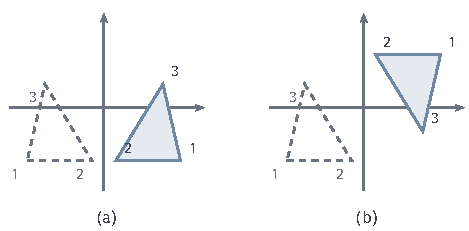
\includegraphics{figures/02-vectors-matrices-and-multivariate-calculus/03-linear-equations-and-optimization/tikz/learning-mechanisms/reflection-versus-rotation.pdf}
  \caption{反射与旋转的几何区别。虚线为原三角形，实色为变换后的位置；(a)关于纵轴反射，行列式为$-1$；(b)绕两轴交点旋转$180^\circ$，行列式为$1$。两幅图仅用于说明允许变换集合的不同，不表示给定矩阵的最优逼近结果。}
  \label{fig:solver-reflection-versus-rotation}
\end{figure}

\paragraph{$s=-1$时原来的上界取不到}
若$s=-1$，$\bm U\bm V^\top$不可行，需要新的上界。仍令$\bm Z=\bm U^\top\bm R\bm V$。对任一旋转$\bm R$，$\bm Z$正交，且
\[
 \det\bm Z=\det\bm U\cdot\det\bm R\cdot\det\bm V=s=-1 .
\]
上一小节的上界依赖$\bm Z=\bm I$可以取到；现在$\det\bm I=1$，这已不可能。

先看$d=2$。行列式为$-1$的二阶正交矩阵都形如
\[
 \bm Z=\begin{bmatrix}\cos\theta&\sin\theta\\\sin\theta&-\cos\theta\end{bmatrix},
\]
它是关于一条直线的反射。代入上一小节的目标，
\[
 \operatorname{tr}(\bm Z^\top\bm\Sigma)=\sigma_1\cos\theta-\sigma_2\cos\theta=(\sigma_1-\sigma_2)\cos\theta .
\]
由$\sigma_1\geq\sigma_2$，它在$\theta=0$处取最大值$\sigma_1-\sigma_2$，这时
\[
 \bm Z=\begin{bmatrix}1&0\\0&-1\end{bmatrix}.
\]
与无约束的上界$\sigma_1+\sigma_2$相比，迹少了$2\sigma_2$：两个对角元不能都取$1$，较小奇异值对应的那个对角元被迫取$-1$。这个例子中$\operatorname{tr}\bm Z=0=d-2$，下面的引理说明一般情形也如此。

\begin{lemma}[行列式为负的正交矩阵的迹]
\label{lem:matrix-approximation-reflection-trace}
设$\bm Z\in\mathbb R^{d\times d}$正交且$\det\bm Z=-1$，则存在单位向量$\bm x$使$\bm Z\bm x=-\bm x$，并且$\operatorname{tr}\bm Z\leq d-2$。
\end{lemma}
\begin{proof}
先证$-1$是特征值。由$\bm Z^\top\bm Z=\bm I$，
\[
 \bm Z+\bm I=\bm Z(\bm I+\bm Z^\top)=\bm Z(\bm I+\bm Z)^\top .
\]
取行列式得
\[
 \det(\bm Z+\bm I)=\det\bm Z\cdot\det(\bm I+\bm Z)=-\det(\bm Z+\bm I),
\]
所以$\det(\bm Z+\bm I)=0$，存在单位向量$\bm x$使$\bm Z\bm x=-\bm x$。再由
\[
 \bm x=\bm Z^\top\bm Z\bm x=-\bm Z^\top\bm x
\]
得$\bm Z^\top\bm x=-\bm x$。

$d=1$时$\bm Z=(-1)$，$\operatorname{tr}\bm Z=-1=d-2$。设$d\geq2$，把$\bm x$扩充为$\mathbb R^d$的标准正交基，排成正交矩阵$\bm Q=[\bm x,\bm Q_2]$。由$\bm Z\bm x=-\bm x$与$\bm Z^\top\bm x=-\bm x$，非对角块为零：
\[
 \bm Q_2^\top\bm Z\bm x=-\bm Q_2^\top\bm x=\bm0,\qquad
 \bm x^\top\bm Z\bm Q_2=(\bm Z^\top\bm x)^\top\bm Q_2=\bm0 .
\]
于是
\[
 \bm Q^\top\bm Z\bm Q=\begin{bmatrix}-1&\bm0\\\bm0&\bm Z_2\end{bmatrix},\qquad\bm Z_2=\bm Q_2^\top\bm Z\bm Q_2 .
\]
左端是正交矩阵的乘积，仍正交，所以$\bm Z_2$的各列是单位向量，对角元都不超过$1$，$\operatorname{tr}\bm Z_2\leq d-1$。迹在相似变换下不变，故
\[
 \operatorname{tr}\bm Z=-1+\operatorname{tr}\bm Z_2\leq d-2 .
\]
\end{proof}

用特征值的语言看，同一结论是这样的。实正交矩阵的特征值模都为$1$：非实特征值成共轭对出现，每对的乘积为$1$、实部之和不超过$2$；实特征值只能是$\pm1$。行列式等于全部特征值之积，为$-1$时特征值$-1$必出现奇数次，至少一次。迹等于特征值之和，于是至多为$(d-1)\cdot1+(-1)=d-2$。上面的证明只用实向量完成了同一论证。

\paragraph{修正最小奇异方向}
有了引理，就可以像$d=2$时那样估计迹的损失。把无约束上界与目标相减，
\[
 \sum_{i=1}^d\sigma_i-\operatorname{tr}(\bm Z^\top\bm\Sigma)=\sum_{i=1}^d\sigma_i(1-z_{i,i}).
\]
每个$1-z_{i,i}$都非负，由引理，它们的和是$d-\operatorname{tr}\bm Z\geq2$。损失是这些量以奇异值为权重的和，而每个权重都不小于最小奇异值$\sigma_d$，所以损失至少是
\[
 \sigma_d(d-\operatorname{tr}\bm Z)\geq2\sigma_d .
\]
这个下界在缺口全部集中于最后一个对角元时取到：$z_{d,d}=-1$，$1-z_{d,d}=2$，其余对角元都等于$1$。相应的$\bm Z$是
\begin{equation}
 \bm D_s=\operatorname{diag}(1,\ldots,1,s),
 \label{eq:matrix-approximation-rotation-correction}
\end{equation}
即只把最后一个对角元改为$s=-1$。换回原变量，最优旋转是$\bm R_\star=\bm U\bm D_s\bm V^\top$。$s=1$时$\bm D_s=\bm I$，这个公式也包含了行列式约束不起作用的情形。

\begin{theorem}[最佳旋转逼近]
\label{thm:matrix-approximation-best-rotation}
设$\bm A\in\mathbb R^{d\times d}$有SVD$\bm A=\bm U\bm\Sigma\bm V^\top$，$\sigma_1\geq\cdots\geq\sigma_d\geq0$，$s=\det(\bm U\bm V^\top)$，$\bm D_s=\operatorname{diag}(1,\ldots,1,s)$。则对一切满足$\bm R^\top\bm R=\bm I$、$\det\bm R=1$的$\bm R$，
\begin{equation}
 \operatorname{tr}(\bm R^\top\bm A)\leq\sum_{i=1}^{d-1}\sigma_i+s\,\sigma_d ,
 \label{eq:matrix-approximation-rotation-trace-bound}
\end{equation}
等号由$\bm R_\star=\bm U\bm D_s\bm V^\top$取到。因此
\begin{equation}
 \min_{\bm R^\top\bm R=\bm I,\ \det\bm R=1}\lVert\bm A-\bm R\rVert_{\mathrm F}^2
 =\sum_{i=1}^{d-1}(\sigma_i-1)^2+(\sigma_d-s)^2 .
 \label{eq:matrix-approximation-rotation-min-error}
\end{equation}
\end{theorem}
\begin{proof}
$\bm R_\star$是正交矩阵的乘积，仍正交，且$\det\bm R_\star=\det\bm U\cdot s\cdot\det\bm V=s^2=1$，所以它是旋转。

$s=1$时$\bm D_s=\bm I$，上界就是定理~\ref{thm:ls-best-orthogonal-approximation}对全部正交矩阵给出的$\sum_i\sigma_i$，在旋转中自然成立，且由$\bm R_\star=\bm U\bm V^\top$取到。

设$s=-1$。对任一旋转$\bm R$，令$\bm Z=\bm U^\top\bm R\bm V$，则$\det\bm Z=-1$，由引理~\ref{lem:matrix-approximation-reflection-trace}，$\operatorname{tr}\bm Z\leq d-2$。与上一小节相同，$\operatorname{tr}(\bm R^\top\bm A)=\sum_i\sigma_iz_{i,i}$。由$|z_{i,i}|\leq1$得$1-z_{i,i}\geq0$，又$\sigma_i\geq\sigma_d$，所以
\[
 \begin{aligned}
 \sum_{i=1}^d\sigma_i-\operatorname{tr}(\bm R^\top\bm A)
 &=\sum_{i=1}^d\sigma_i(1-z_{i,i})
 \geq\sigma_d\sum_{i=1}^d(1-z_{i,i})\\
 &=\sigma_d(d-\operatorname{tr}\bm Z)\geq2\sigma_d ,
 \end{aligned}
\]
即
\[
 \operatorname{tr}(\bm R^\top\bm A)\leq\sum_{i=1}^{d-1}\sigma_i-\sigma_d .
\]
$\bm R=\bm R_\star$时$\bm Z=\bm D_s$，迹恰为$\sum_{i<d}\sigma_i-\sigma_d$，等号成立。

最后代入展开式。由$\lVert\bm A\rVert_{\mathrm F}^2=\sum_i\sigma_i^2$与$s^2=1$，
\[
 \sum_{i=1}^d\sigma_i^2+d-2\Bigl(\sum_{i=1}^{d-1}\sigma_i+s\sigma_d\Bigr)
 =\sum_{i=1}^{d-1}(\sigma_i-1)^2+(\sigma_d-s)^2 .
\]
\end{proof}

\paragraph{修正的代价}
修正只发生在最小奇异方向上。$\bm R_\star=\bm U\bm D_s\bm V^\top$与无约束解$\bm U\bm V^\top$的差别，是把最后一对奇异方向的配对改为$\bm v_d\mapsto s\bm u_d$。若把符号改放在第$i$个方向上，同样得到旋转，但迹损失$2\sigma_i$；定理证明中的不等式说明，任何旋转的迹损失都至少是$2\sigma_d$，所以放在最小奇异方向上损失最少。

$s=-1$时，最小平方误差比无行列式约束时增加
\begin{equation}
 (\sigma_d+1)^2-(\sigma_d-1)^2=4\sigma_d .
 \label{eq:matrix-approximation-rotation-cost}
\end{equation}
$\bm A$可逆时，$\det\bm A=\det\bm U\det\bm\Sigma\det\bm V$且$\det\bm\Sigma>0$，所以$s$就是$\det\bm A$的符号，与所取的SVD无关：$\det\bm A>0$时约束不起作用，$\det\bm A<0$时代价为$4\sigma_d$。

$\sigma_d=0$时，$s$依赖SVD的选取：把$\bm u_d$换成$-\bm u_d$不改变$\bm A$，却改变$\det\bm U$的符号。但这时$(\sigma_d-s)^2=1$与$s$无关，旋转约束的代价为零。两种选取还给出同一个$\bm R_\star$，因为符号同时出现在$\bm u_d$与$s$中，乘积$s\bm u_d$不变。

\paragraph{唯一性}
唯一性分两种情形说明。第一种，$\bm A$可逆且$s=1$：无约束问题的唯一解$\bm W$本身是旋转，所以它也是旋转约束下的唯一解。

第二种，$\sigma_{d-1}>\sigma_d$。若$\sigma_d>0$且$s=-1$，定理证明中的不等式取等要求$(\sigma_i-\sigma_d)(1-z_{i,i})=0$，从而$i<d$时$z_{i,i}=1$，$\bm Z$的前$d-1$列是$\bm e_1,\ldots,\bm e_{d-1}$；最后一列只能是$\pm\bm e_d$，行列式为$-1$又迫使它为$-\bm e_d$，即$\bm Z=\bm D_s$。

若$\sigma_d=0$，先取使$s=1$的SVD，取等要求$z_{i,i}=1$（$i<d$），同理$\bm Z=\operatorname{diag}(1,\ldots,1,\pm1)$，而$\det\bm Z=s=1$，故$\bm Z=\bm I$。两种情况下最优旋转都唯一。

最小奇异值重复且$s=-1$，或$\operatorname{rank}\bm A\leq d-2$时，最优旋转可以不唯一，例子见本小节的算法分析。

\subsubsection{算法实现}

计算在上一小节的基础上增加两步：求出符号$s$，再在最小奇异方向上作修正。下面写出用到的变量与各步计算，并用以下示例逐步演示。

\begin{example}[对角矩阵的旋转逼近]
\label{ex:matrix-approximation-rotation-diagonal}
求离
\[
 \bm A=\begin{bmatrix}3&0\\0&-1\end{bmatrix}
\]
最近的旋转。$\det\bm A=-3<0$，上一小节的无约束解包含反射，行列式约束会起作用。下面的逐步执行给出$\bm R_\star$与平方误差，并与无约束解比较。
\end{example}

\paragraph{变量}
\begin{itemize}
 \item $\bm A\in\mathbb R^{d\times d}$：给定的方阵。
 \item $\bm U,\bm\Sigma,\bm V$：$\bm A$的完整方阵SVD，奇异值按非增顺序排列。
 \item $s=\det\bm U\det\bm V$：无约束解$\bm U\bm V^\top$的行列式。
 \item $\bm D_s=\operatorname{diag}(1,\ldots,1,s)$：最小奇异方向上的符号修正。
 \item $\bm R_\star$：所求的最优旋转。
\end{itemize}

\paragraph{输入与预处理}
输入方阵$\bm A$，预处理是求它的完整方阵SVD，并把奇异值按非增顺序排列，使最后一列$\bm u_d$、$\bm v_d$对应最小奇异值。符号修正要放在这一对方向上，排序不能省略。

例中
\[
 \bm A^\top\bm A=\begin{bmatrix}9&0\\0&1\end{bmatrix},
\]
可取$\bm V=\bm I$，奇异值$\sigma_1=3\geq\sigma_2=1$。由$\bm u_i=\bm A\bm v_i/\sigma_i$，
\[
 \bm u_1=\frac13\begin{bmatrix}3\\0\end{bmatrix}=\begin{bmatrix}1\\0\end{bmatrix},\qquad
 \bm u_2=\frac11\begin{bmatrix}0\\-1\end{bmatrix}=\begin{bmatrix}0\\-1\end{bmatrix},
\]
于是
\[
 \bm U=\begin{bmatrix}1&0\\0&-1\end{bmatrix},\qquad
 \bm\Sigma=\begin{bmatrix}3&0\\0&1\end{bmatrix},\qquad
 \bm V=\bm I ,
\]
核对$\bm U\bm\Sigma\bm V^\top=\operatorname{diag}(3,-1)=\bm A$。

\paragraph{计算步骤}
\begin{enumerate}
 \item \textbf{计算符号。}按式~\eqref{eq:matrix-approximation-rotation-sign}计算
 \[
  s=\det\bm U\det\bm V .
 \]
 例中
 \[
  s=(-1)\cdot1=-1 .
 \]
 作为对照，无约束的最优正交矩阵是$\bm U\bm V^\top=\operatorname{diag}(1,-1)$，它是关于横轴的反射，平方误差为
 \[
  \lVert\operatorname{diag}(2,0)\rVert_{\mathrm F}^2=4=(3-1)^2+(1-1)^2 .
 \]

 \item \textbf{构造修正矩阵。}按式~\eqref{eq:matrix-approximation-rotation-correction}取
 \[
  \bm D_s=\operatorname{diag}(1,\ldots,1,s).
 \]
 例中
 \[
  \bm D_s=\begin{bmatrix}1&0\\0&-1\end{bmatrix}.
 \]

 \item \textbf{相乘得最优旋转。}计算
 \begin{equation}
  \bm R_\star=\bm U\bm D_s\bm V^\top .
  \label{eq:matrix-approximation-rotation-optimum}
 \end{equation}
 例中
 \[
  \bm R_\star=\begin{bmatrix}1&0\\0&-1\end{bmatrix}\begin{bmatrix}1&0\\0&-1\end{bmatrix}=\begin{bmatrix}1&0\\0&1\end{bmatrix}.
 \]

 \item \textbf{核验。}同时检查三项：$\bm R_\star^\top\bm R_\star=\bm I$，$\det\bm R_\star=1$，误差平方等于$\sum_{i<d}(\sigma_i-1)^2+(\sigma_d-s)^2$。

 例中$\bm R_\star=\bm I$，前两项显然成立；残差为$\bm A-\bm R_\star=\operatorname{diag}(2,-2)$，
 \[
  \lVert\bm A-\bm R_\star\rVert_{\mathrm F}^2=4+4=8=(3-1)^2+(1+1)^2 .
 \]
 比无约束时多$4=4\sigma_2$。
\end{enumerate}

最终得到离$\bm A$最近的旋转
\[
 \bm R_\star=\begin{bmatrix}1&0\\0&1\end{bmatrix},
\]
平方误差为$8$。

二阶旋转可以全部写出来，用于独立核对。对
\[
 \bm R=\begin{bmatrix}\cos\theta&-\sin\theta\\\sin\theta&\cos\theta\end{bmatrix},
\]
按元素求和得
\[
 \operatorname{tr}(\bm R^\top\bm A)=3\cos\theta-\cos\theta=2\cos\theta ,
\]
它只在$\theta=0$处取最大值$2=\sigma_1-\sigma_2$。所以$\bm R_\star=\bm I$是唯一的最优旋转，与$\sigma_1>\sigma_2$时的唯一性一致。

\subsubsection{算法分析}

\paragraph{计算代价}
与无约束情形相比，额外的工作只是求两个正交矩阵的行列式与一次对角缩放，主要代价仍是SVD。是否需要修正完全由$s$决定，不必比较多个候选。

\paragraph{最优旋转不唯一的情形}
最小奇异值重复时，唯一性可能失败。取$\bm A=\operatorname{diag}(1,-1)$，奇异值为$1,1$，$s=-1$。对上面的任一二阶旋转，
\[
 \operatorname{tr}(\bm R^\top\bm A)=\cos\theta-\cos\theta=0 ,
\]
由展开式~\eqref{eq:matrix-approximation-orthogonal-expansion}，所有旋转的误差平方都是
\[
 \lVert\bm A\rVert_{\mathrm F}^2+2-0=4 ,
\]
与公式$(1-1)^2+(1+1)^2=4$一致，但最优旋转有无穷多个。

$\operatorname{rank}\bm A\leq d-2$时也有类似的自由度，例如$\bm A=\bm0$时每个旋转都最优。

\paragraph{接近奇异时的敏感性}
最小奇异值接近零时，$s$对$\bm A$的微小变化很敏感：$\det\bm A$接近零，它的符号可能被扰动改变，最优旋转随之跳到另一个。但对同一个$\bm A$，两种符号给出的误差平方恰好相差$4\sigma_d$，这时也很小，最优误差本身随$\bm A$连续变化。所以这种情形下应报告最优误差，而不应把所得的旋转当作稳定的估计。
